\section[\thesection \  Positionieren von Einzelachsen]{Positionieren von
Einzelachsen}\label{sec:positioneinzelachsen}
%
%--------------------------------------------------------------------
%
\subsection[\thesection .\thesubsection \ 
Bewegungsprofil]{Bewegungsprofil}\label{sec:bewegungsprofil}
%
\begin{frame}{Einfaches Streckenmodell}
%
Einfaches Streckenmodell für die prinzipiellen Zusammenhänge
%
\begin{itemize}
  \item Kein Getriebe
  \item Starre Welle
  \item $J_G=J_M+J_L$
\end{itemize}
%
\begin{center}
%
\begin{tikzpicture}
%
\draw(0,0)node[rectangle,minimum width = 1.8cm,minimum height =
1.2cm,draw](m2n){};
\draw(m2n.south west)--(m2n.north east);
\draw(m2n.north west)node[above]{$\dfrac{1}{J_G}$};
%
\draw($(m2n.east)+(1,0)$)node[rectangle,minimum width = 1.8cm,minimum height =
1.2cm,draw,anchor = west](n2x){};
\draw(n2x.south west)--(n2x.north east);
%
\draw($(m2n.west)+(-1,0)$)node[circle,minimum width = 0.2cm,draw](deltam){};
%
%---------------
%
\draw[-latex](m2n.east)--(n2x.west)node[pos = 0.5,above]{$\Omega$};
\draw[-latex](deltam.east)--(m2n.west);
%
\coordinate (mm) at ($(deltam.west)+(-1,0)$);
\coordinate (ml) at ($(deltam.north)+(0,1)$);
\coordinate (xist) at ($(n2x.east)+(1,0)$);
%
\draw[-latex] (mm)node[above right]{$M_M$}--(deltam.west);
\draw[-latex] (ml)node[below left]{$M_L$}--(deltam.north)node[above left]{$-$};
\draw[-latex] (n2x.east)--(xist)node[above left]{$\varphi$};
%
\end{tikzpicture}
%
\end{center}
%

\vspace{12pt}

Für die folgenden Überlegungen gilt~$M_L=0$.

\vspace{6pt}

Bezeichung: $\ddot \varphi =\dot \Omega = \alpha$

\vfill

%
\end{frame}
%
%--------------------------------------------------------------------
%
\begin{frame}{Drehmomentvorgabe}
%
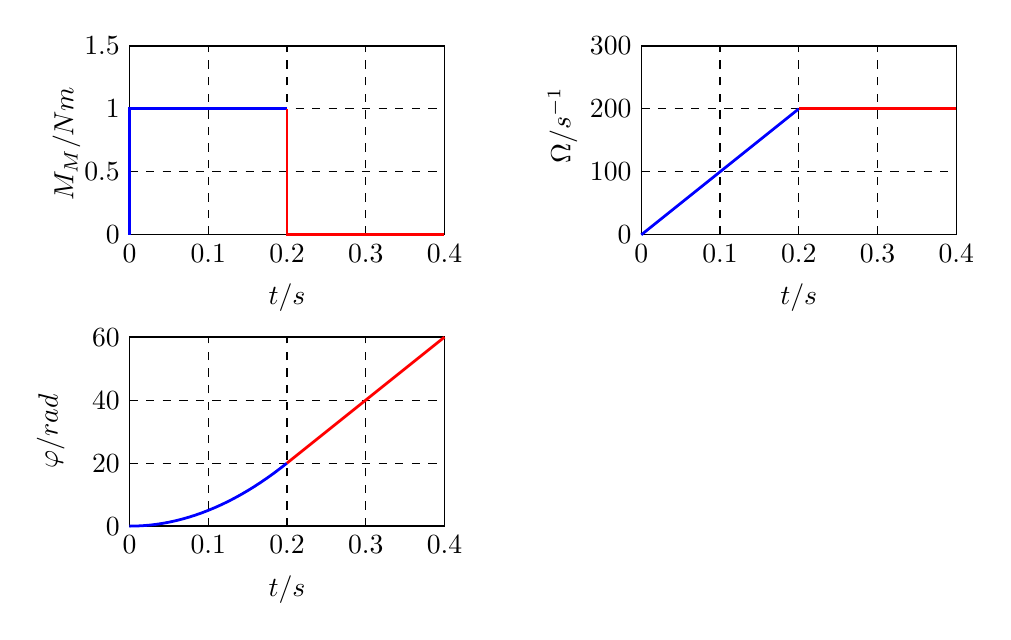
\begin{tikzpicture}
%
%Bewegungsprofil fuer J = 10e-4kgm^2
%
\draw[dashed,ystep=0.8] (0,0) grid (4,2.4);
\draw[line width = 0.5pt] (0,0) rectangle (4,2.4);
%
\draw(-0.8,2)node[left,rotate = 90]{$M_M/Nm$};
\foreach \y/\ytext in {0/0,0.8/0.5,1.6/1,2.4/1.5}
\draw(0,\y)node[left]{$\ytext$};
%
\draw(2,-0.5)node[below]{$t/s$};
\foreach \x/\xtext in {0/0,1/0.1,2/0.2,3/0.3,4/0.4}
\draw(\x,0)node[below]{$\xtext$};
%
%Drehmoment
%
\visible<2->{\draw[line width = 1pt,color = blue](0,0)--(0,1.6)--(2,1.6);}
\visible<3->{\draw[line width = 1pt,color = red](2,1.6)--(2,0)--(4,0);}
%
%--------------------------------------------------------------------
%
\begin{scope}[xshift = 6.5cm]
%
\draw[dashed,ystep=0.8] (0,0) grid (4,2.4);
\draw[line width = 0.5pt] (0,0) rectangle (4,2.4);
%
\draw(-1,2)node[left,rotate = 90]{$\Omega/s^{-1}$};
\foreach \y/\ytext in {0/0,0.8/100,1.6/200,2.4/300}
\draw(0,\y)node[left]{$\ytext$};
%
\draw(2,-0.5)node[below]{$t/s$};
\foreach \x/\xtext in {0/0,1/0.1,2/0.2,3/0.3,4/0.4}
\draw(\x,0)node[below]{$\xtext$};
%
%Omega
%
\visible<2->{\draw[line width = 1pt,color = blue](0,0)--(2,1.6);}
\visible<3->{\draw[line width = 1pt,color = red](2,1.6)--(4,1.6);}
%
\end{scope}
%
%--------------------------------------------------------------------
%
\begin{scope}[yshift = -3.7cm]
%
\draw[dashed,ystep=0.8] (0,0) grid (4,2.4);
\draw[line width = 0.5pt] (0,0) rectangle (4,2.4);
%
\draw(-1,1.8)node[left,rotate = 90]{$\varphi/\text{rad}$};
\foreach \y/\ytext in {0/0,0.8/20,1.6/40,2.4/60}
\draw(0,\y)node[left]{$\ytext$};
%
\draw(2,-0.5)node[below]{$t/s$};
\foreach \x/\xtext in {0/0,1/0.1,2/0.2,3/0.3,4/0.4}
\draw(\x,0)node[below]{$\xtext$};
%
%\varphi
%
\visible<2->{\draw[line width = 1pt,color = blue,domain = 0:2]plot
(\x,{25*0.8*(\x*\x/100)});} %Skalierung der y-Achse auf 0.8 ^=20
\visible<3->{\draw[line width = 1pt,color =red](2,0.8)--(4,2.4);}
%
\end{scope}
%
\end{tikzpicture}
%
\end{frame}
%
%--------------------------------------------------------------------
%
\begin{frame}{Positionsvorgabe}
%
\begin{block}{Gegeben:}
%
\begin{columns}[T]
%
\column{0.35\textwidth}
Startposition $\varphi(t_0)=\varphi_0$
%
\column{0.6\textwidth}
Zielposition $\varphi(t_0+T_Z)=\varphi_Z$
%
\end{columns}
%
\end{block}
%
\begin{block}{Gesucht:}
%
\begin{columns}
%
\column{0.25\textwidth}
Bewegungsprofil:
%
\column{0.7\textwidth}
%
\begin{align}
%
\left. \begin{array}{l} \Omega(t) \\ M(t)\end{array}\right\} &\qquad \text{so
dass die Zielposition~$\varphi_Z$ erreicht wird}\nonumber
%
\end{align}
%
\end{columns}
%
\end{block}
%
Mögliche Vorgaben/Randbedingungen:
%
\begin{itemize}
  \item Vorgegebene Grenzwerte $\Omega_{\max}$, $\alpha_{\max}$, $M_{\max}$
  \item Randwerte $\Omega(t_0)$, $\Omega(t_0+T_Z)$, $\alpha(t_0)$,
  $\alpha(t_0+T_Z)$
  \item Dauer des Positioniervorgangs
  \begin{itemize}
    \item $T_Z$ vorgegeben
    \item $T_Z$ frei
  \end{itemize}
\end{itemize}
%
\end{frame}
%
%
%--------------------------------------------------------------------
%
\subsection[\thesection .\thesubsection \ 
Lageregelkreis]{Lageregelkreis}\label{sec:lageregelkreis}
%
%--------------------------------------------------------------------
%
\begin{frame}{Varianten der Positionierung}
%
\begin{block}{Absolutes Positionieren}
%
Die Zielposition bezieht sich immer auf den gleichen Referenzwert.
%
\end{block}
%
%
\begin{block}{Relatives Positionieren}
%
Die Zielposition bezieht sich immer auf die aktuelle Position.
%
\end{block}
%
\alert{Problem:} Aufgrund begrenzter  Genauigkeit pflanzen sich Fehler fort.
%
\begin{columns}[T]
%
\column{0.55\textwidth}
%
\begin{block}{Beispiel:}
%
Geberauflösung 1024 Striche / Umdr.\ 

Relatives Positionieren um jeweils 10 grad
%
\end{block}
%

\vspace{12pt}

\visible<2->{\alert{Abhilfe:} Korrektur durch Resteverwaltung}
%
\column{0.05\textwidth}

\column{0.35\textwidth}
%
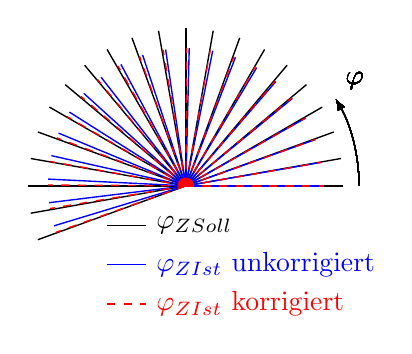
\begin{tikzpicture}
%
%Wunsch
%
\foreach \x in
{0,10,20,30,40,50,60,70,80,90,100,110,120,130,140,150,160,170,180,190,200}
%
\draw[line width =0.5pt](0,0)--(\x:2);
%
%Ohne Korrektur
%
\foreach \x in
{0,9.84375,19.6875,29.53125,39.375,49.21875,59.0625,68.90625,78.75,88.59375,98.4375,108.28125,118.125,127.96875,137.8125,147.65625,157.5,167.34375,177.1875,187.03125,196.875}
%
\draw[blue,line width =0.5pt](0,0)--(\x:1.75);
%
%Mit Korrektur
%
\foreach \x in
{0,9.84375,19.6875,29.53125,39.726562,49.570312,59.765625,69.609375,
79.804688,89.648438,99.492188,109.6875,119.53125,129.72656,139.57031,
149.76562,159.60938,169.80469,179.64844,189.49219,199.6875}
%
\visible<2->{\draw[red,line width =0.5pt,dashed](0,0)--(\x:1.75);}
%
\draw[-latex] (0:2.2) arc (0:30:2.2)node[above right]{$\varphi$};
%
%Legende
%
\draw[line width =0.5pt]
(-1,-0.5)--(-0.5,-0.5)node[right]{$\varphi_{Z\text{Soll}}$}; 
\draw[blue,line width =0.5pt]
(-1,-1)--(-0.5,-1)node[right]{$\varphi_{Z\text{Ist}}$ unkorrigiert}; 
%
\visible<2->{\draw[red,line width
=0.5pt,dashed] (-1,-1.5)--(-0.5,-1.5)node[right]{$\varphi_{Z\text{Ist}}$
korrigiert};}
%
\end{tikzpicture}
%
\end{columns}
%
\end{frame}